\documentclass[10pt]{article}
% for pdflatex
\usepackage[utf8]{inputenc}
% for hyperlink
\usepackage{hyperref}
\hypersetup{
    colorlinks=true,
    linkcolor=blue,
    filecolor=magenta,      
    urlcolor=cyan,
}
% for custom enum
\usepackage{enumitem}
% for removing alinea begin of paragraph
\usepackage{parskip}
\usepackage{array, xcolor, graphicx}
\usepackage[a4paper, margin=1cm]{geometry}
\title{\bfseries\Huge Blockchain Engineer\vspace{-4ex}}
% no author
\author{\bfseries\Huge \vspace{-4ex}}
% no date
\date{}
% custom for column style
\definecolor{lightgray}{gray}{0.8}
% custom for column type
\newcolumntype{L}{p{0.18\textwidth}}
% custom for column type
\newcolumntype{R}{p{0.75\textwidth}}
% custom for column type
\newcommand\VRule{\color{lightgray}\vrule width 2pt}
% for bullet point outside of list
\newcommand{\tabitem}{~~\llap{$\rightarrow$}~~}
\begin{document}

\begin{minipage}[t]{0.80\textwidth}
\textbf{Mohamed Amine LEGHERABA}\\
24 years old\\
92 bis rue Rouget de Lisle, Bezons, France\\
+33 (0) 6 30 82 90 00\\
\href{mailto:mlegheraba@protonmail.com}{mlegheraba@protonmail.com}\\
\url{https://github.com/MohamedLEGH} \\

{\bf French}: native \\
{\bf Anglais}: fluent (TOIEC: 935) \\
\end{minipage}
\begin{minipage}[t]{0.20\textwidth}
\vspace{-3ex}
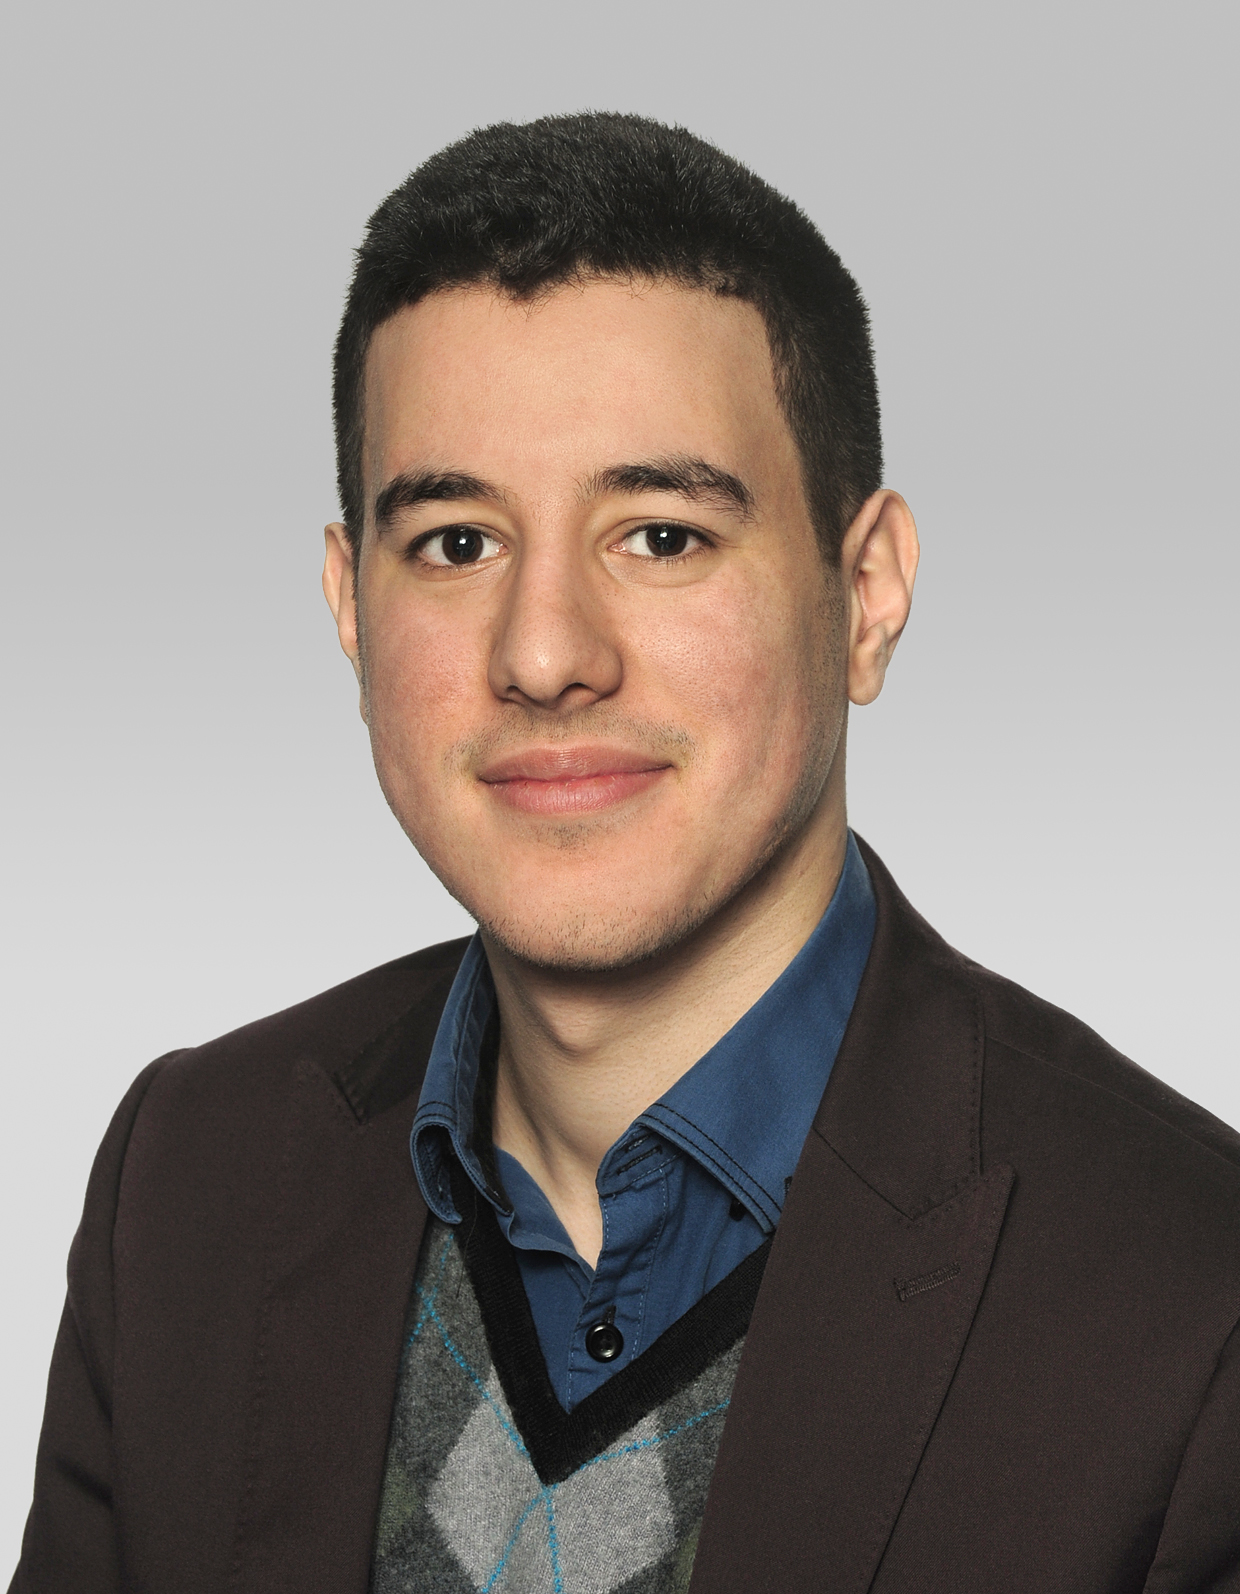
\includegraphics[width=3cm]{Legheraba-Mohamed.jpg}
\end{minipage}
\vspace{-8ex}
% to make maketitle work without begin of page
{\let\newpage\relax\maketitle}
% to remove page number
\thispagestyle{empty}

\vspace{-8ex}

\section*{Formation}
\begin{tabular}{L!{\VRule}R}
\textbf{\textit{2015--2018}} & \textbf{Selective engineering school Polytech Sorbonne}, speciality \textit{Applied mathematics and computer science}. Erasmus semester at TU Delft, Netherlands, Winter 2017.\\[0.75cm]
\textbf{\textit{2013--2015}} & \textbf{Selective engineering school Polytech Sorbonne},  \textit{PeiP} (an intensive 2-year preparation course for the competitive
entrance to French engineering schools)\\[0.75cm]
\textbf{\textit{2013}}&\textbf{Secondary education leaving certificate}. In Science. With honours, Lycée Chaptal. \\
\end{tabular}
 

\section*{Work Experience}
\begin{tabular}{L!{\VRule}R}
\textbf{\textit{Since 2019}}& 
\includegraphics[width=2cm]{SIA_logo.png} \hspace{0.2cm} {\bf Blockchain Developer, Sia Partners} \\[0.25cm]

& \tabitem \small{\textbf{Development of blockchain applications for Sia Partners customers} (Corda network for an asset manager, mobile payment application in cryptocurrencies, ...)}

\\[0.20cm]
& \tabitem \small{\textbf{Study of case studies on the use of the blockchain with business teams} (food traceability, recording of clinical trials, time-stamping of IoT sensor data, ...)}

\\[0.20cm]
& \tabitem \small{\textbf{R\&D watch on blockchain and cryptocurrencies} (study of Liquid, Libra and TON blockchain networks, Lightning Network, Taproot and Multi-Party Computation technologies, ...)}

\\[0.20cm]
& \tabitem \small{\textbf{Writing articles} (\href{https://telecom.sia-partners.com/20191024/la-blockchain-catalyseur-de-la-decentralisation-et-de-la-securisation-des-reseaux-5g}{\textit{Blockchain \& 5G}}, \href{https://telecom.sia-partners.com/20200212/entretien-avec-pierre-noizat-bitcoin-et-cryptomonnaies-point-de-vue-de-la-premiere}{\textit{Interview with Pierre Noizat}}, ...)}

\\[0.20cm]
& \tabitem \small{\textbf{Course \textit{Programming a blockchain}} (\href{https://github.com/MohamedLEGH/tutoriel-blockchain-creation-bootstrap}{Polytech Sorbonne}, \href{https://github.com/MohamedLEGH/tutoriel-blockchain-MinesBootstrap}{Mines St Etienne}, ...)}

\\[0.20cm]
\textbf{\textit{March--September 2018}}& 
\includegraphics[width=1.5cm]{ofi-am.png} \hspace{0.2cm} {\bf R\&D watch intern, Development Department, OFI AM, 6 mois}.\\
& \small{Watch around Blockchain technologies, task automation with Airflow, application containerisation with Docker and system supervision with Tableau Server.} \\

\end{tabular}
 
 
\section*{Competences}
\begin{tabular}{ l l }
\textbf{Blockchain}: \textbf{\textit{Bitcoin}}, \textbf{\textit{Ethereum}}, Hyperledger, Corda & \textbf{Databases}: MySQL, \textbf{\textit{PostgreSQL}}, Neo4J \\[0.1cm]
\textbf{Smart contracts}: \textbf{\textit{Solidity}}, Bitcoin Script, Chaincodes & \textbf{Programming}: \textbf{\textit{Python}}, \textbf{\textit{JavaScript}}, C/C++, R  \\[0.1cm]
\textbf{System tools}: \textbf{\textit{Shell}}, Linux, Git, Bash, \textbf{\textit{Docker}} & \textbf{Frameworks}: \textbf{\textit{ReactJS}}, \textbf{\textit{Nodejs}}, Flask, PyQt, R Shiny \\[0.1cm]
\textbf{Mathematics}: Cryptography, Statistics, Graphs & \textbf{Computer Science}: Algorithmic, Parallelism, Compilers \\[0.1cm]
\textbf{Protocols}: \textbf{\textit{Lightning Network}}, IPFS, BitTorrent & \textbf{Cloud}: Google, AWS, Azure, Gitlab CI/CD, Kubernetes
\end{tabular}

\section*{Volunteer Experience}
\begin{tabular}{L!{\VRule}R}
\textbf{\textit{Since 2018}} & Association \textbf{Le Trait D’Union}, Homework help for high school and college students. Writing grant applications. \\[0.75cm]

\textbf{\textit{2014--2017}} & Student association \textbf{Averroès}, Food donations for students, treasurer then president. \\
\end{tabular}
\section*{Interests}
\hspace*{1ex} \textbf{Electronics} (retrogaming console with a Raspberry Pi, fan control using a transistor, ...) \\
\hspace*{1ex} \textbf{Study of socio-economic doctrines} (liberalism, Austrian school of economics, anarchism, technoethics, ...) \\
\end{document}
